% ============================================================
% analy 报告 — dev78_1 完整复测与深化（参数优化验证 + 全套图表）
% 编译: xelatex 两遍；交付前 Overfull 计数必须为 0
% ============================================================
\documentclass[UTF8]{ctexart}
\usepackage[margin=2.5cm]{geometry}
\usepackage{amsmath}
\usepackage{microtype}
\usepackage{listings}
\usepackage{xcolor}
\usepackage{booktabs}
\usepackage{longtable}
\usepackage{xltabular}
\usepackage{tabularx}
\usepackage{hyperref}
\usepackage{fancyhdr}
\usepackage[most]{tcolorbox}
\usepackage{titlesec}
\usepackage{graphicx}

% ===== 色板 =====
\definecolor{accent}{HTML}{1F4E79}
\definecolor{evidence}{HTML}{1E8449}
\definecolor{reference}{HTML}{8C6D1F}
\definecolor{conclusion}{HTML}{8B1A1A}
\definecolor{codebg}{HTML}{F4F6F7}
\definecolor{struct}{HTML}{3B3B98}
\definecolor{relation}{HTML}{0E7C7B}
\definecolor{idea}{HTML}{B03A2E}
\definecolor{warn}{HTML}{D35400}
\definecolor{hl}{HTML}{FDF6E3}

\setlength{\emergencystretch}{3em}
\hypersetup{colorlinks=true,linkcolor=accent,urlcolor=relation}

\titleformat{\section}{\Large\bfseries\color{accent}}{\thesection}{1em}{}
\titleformat{\subsection}{\large\bfseries\color{struct}}{\thesubsection}{1em}{}
\titleformat{\subsubsection}{\normalsize\bfseries\color{struct!70!black}}{\thesubsubsection}{1em}{}

\newtcolorbox{conclbox}{breakable,colback=conclusion!6,colframe=conclusion,title=结论}
\newtcolorbox{refbox}{breakable,colback=reference!6,colframe=reference,title=参考背景}
\newtcolorbox{ideabox}{breakable,colback=idea!6,colframe=idea,title=项目思路}
\newtcolorbox{warnbox}{breakable,colback=warn!6,colframe=warn,title=局限与风险}
\newtcolorbox{keybox}{breakable,colback=hl,colframe=accent,title=要点}

\lstset{
  basicstyle=\ttfamily\footnotesize,
  backgroundcolor=\color{codebg},
  frame=single,
  language=python,
  firstnumber=auto,
  keywordstyle=\color{accent}\bfseries,
  commentstyle=\color{evidence!70!black},
  stringstyle=\color{struct},
  breaklines=true,
  breakatwhitespace=false,
  postbreak=\mbox{\textcolor{accent}{$\hookrightarrow$}\space},
  keepspaces=true,
  columns=flexible,
  numbers=left,numberstyle=\tiny\color{struct!60!black},
}

\title{dev78\_1 --- 参数优化完整复测与深化（r10/r20 验证 + 全套图表与日志）}
\author{opencode analy}
\date{\today}

\begin{document}
\maketitle

\begin{abstract}
本报告对 dev78\_1（logs/dev78\_1/）进行详细分析：它是 dev78 中/大格子
num\_restart 参数优化（r10/r20）的\textbf{完整复测与深化}，参考 logs/dev74
输出形式，归档全部日志、全套图表与详细报告。三视角概览：
\textcolor{struct}{主体结构}为测试套件（main.py 子命令 + 版本目录 + h5py）
叠加 dev74 风格的补充图表层（conv/vram/prof）；
\textcolor{relation}{各部分关系}为 num\_restart → V-cycle 频率 → 粗层求解
次数 → 总时间的主链；\textcolor{idea}{项目思路}为参数优化以实测验证闭环
（PROF 定位 → r 调整 → 双模式确认 → 全套归档）。核心结论：bench 中位
加速比 1.148 → 1.210 → \textbf{1.422}（dev76→dev78→dev78\_1 持续提升）；
8x16x16x16 2L r10 达 1.48（r5 时 0.33-0.69，约 3 倍）；verify 全 PASS。
\end{abstract}

\tableofcontents

% ================= 1 概览 =================
\section{目录概览}
logs/dev78\_1/ 结构（与 dev74 输出形式对齐）：
\begin{lstlisting}[language=bash]
logs/dev78_1/
├── main.py / run-local.sh / AGENTS.md   套件代码
├── dev78_1_report.md                    详细报告（md）
├── docs/                                analy 报告（tex/pdf）
└── v202608160214/                       最终版本目录
    ├── verify.log / clean.log / bench.log / sweep.log   全部日志
    ├── test78_1_verify.h5 / bench.h5 / sweep.h5 / results.h5
    ├── test78_1_budget_16g.h5 / _32g.h5
    ├── test78_1_speedup.png / time.png / sweep.png / hotspot.png
    ├── dev78_1_conv_bench.png / vram_16g.png / vram_32g.png / prof.png
    └── test78_1_tbl_bench.tex / tbl_sweep.tex
\end{lstlisting}

\begin{table}[htbp]\centering
\begin{tabular}{ll}
\toprule
指标 & 实测值 \\
\midrule
bench 中位加速比 & \textbf{1.422} \\
bench 最大加速比 & \textbf{2.271}（8x8x8x16 3L P100x2） \\
sweep 通过率（gate=1.5） & 14/16（best 2.480） \\
verify & 全 PASS \\
图表数 & 8 张 PNG + 2 张 LaTeX 表 \\
日志数 & 4 份（verify/clean/bench/sweep）+ C++ 收敛日志 \\
\bottomrule
\end{tabular}
\caption{dev78\_1 实测统计（数据来源: results.h5 / 文件清单实测）}
\end{table}

% ================= 2 主体结构 =================
\section{主体结构}
\begin{table}[htbp]\centering
\begin{tabularx}{\textwidth}{llX}
\toprule
\textcolor{struct}{层次} & 文件 & \textcolor{struct}{职责} \\
\midrule
入口层 & main.py / run-local.sh & 测试编排（9 子命令） \\
数据层 & test78\_1\_*.h5 & h5py 持久化结果 \\
图表层 & *.png / tbl\_*.tex & 可视化（speedup/time/sweep/hotspot/conv/vram/prof） \\
文档层 & dev78\_1\_report.md / docs/ & 详细报告与 analy \\
\bottomrule
\end{tabularx}
\caption{主体结构分层（数据来源: 全库索引实测）}
\end{table}

\textcolor{struct}{与 dev74 输出对齐}：dev74 有 conv（收敛图）、vram、budget、
speedup 图；dev78\_1 补足 conv\_bench、vram\_16g/32g、prof（PROF 占比），
使图表覆盖从正确性到资源预算的完整维度。

% ================= 3 各部分关系 =================
\section{各部分关系}
\begin{keybox}
\textbf{参数-性能主链:} \textcolor{relation}{num\_restart（V-cycle 频率）→
V-cycle 次数 → 粗层求解次数（fused 38-58ms/次 / 多 block ~117ms/次）→
总求解时间。r5 时 8x16x16x16 2L 的 n\_vcycles 13-44 次爆炸（vcycle 602-2244ms）
→ r10 减半 → 加速比 0.33-0.69 → 1.05-1.48}
\end{keybox}

跨里程碑演进（bench 中位加速比）：dev76（粗层归约优化）1.148 →
dev78（r 参数优化）1.210 → dev78\_1（完整复测）\textbf{1.422}。
每次优化环：PROF\_SECTIONS 定位主导项 → 最小改动 → 双模式（V100/P100x2）
验证 → 归档。

% ================= 4 项目思路 =================
\section{项目思路}
\subsection{设计意图}
\begin{itemize}
\item \textcolor{idea}{实测闭环}：参数调整必须有 PROF 证据与双模式复测；
\item \textcolor{idea}{输出对齐}：参考 dev74 的图表/日志/报告形式，保证
  跨里程碑可比；
\item \textcolor{idea}{图表完整}：从正确性（verify 日志）到性能（bench/sweep
  图）到资源（budget/vram 图）到收敛（conv/prof 图）全覆盖。
\end{itemize}
\subsection{演进脉络}
test12（单线程）→ test13（多线程）→ test14（构建加速）→ dev76（粗层求解
加速）→ dev78（V-cycle 频率优化）→ dev78\_1（完整复测与深化，本次）。
\subsection{典型工作流}
\texttt{run-local.sh → 版本目录 v<ts>/ → main.py 各子命令 → collect/mktable/
plots → make\_extra\_plots.py（conv/vram/prof）→ 报告 md/tex/pdf}。

\begin{ideabox}
项目思路核心：参数优化的价值必须由完整复测证明——verify 正确性 +
bench 性能 + sweep 参数空间 + budget 资源 + conv/prof 收敛性，缺一不可。
\end{ideabox}

% ================= 5 主题分析 =================
\section{主题分析}
\subsection{正确性（verify）}
四合一验证全 PASS：一致性（2xP100 rel=0）、独立问题（|d|=5.67）、
V100 大格子 3L（rel=0）、h5py 4 线程 IO（max\_err=0）。

\subsection{性能（bench）}
\begin{table}[htbp]\centering
\begin{tabular}{lllll}
\toprule
配置 & 设备 & r & speedup & 相对 dev76 \\
\midrule
8x8x8x16 2L & P100x2 & 5 & \textbf{1.94-2.01} & 持平 \\
8x8x8x16 3L & P100x2 & 5 & \textbf{2.14-2.29} & +5\% \\
8x16x16x16 2L & P100x2 & 10 & \textbf{1.05-1.48} & 约 3 倍 \\
8x16x16x16 3L & P100x2 & 10 & \textbf{1.41} & 约 2 倍 \\
16x16x16x16 2L & P100x2 & 20 & \textbf{0.66-0.74} & +12\% \\
16x16x16x16 3L & V100 & 10 & \textbf{1.17} & 持平 \\
8x16x16x16 3L & V100 & 10 & \textbf{1.42} & 持平 \\
\bottomrule
\end{tabular}
\caption{bench 实测（数据来源: test78\_1\_bench.h5）}
\end{table}

\subsection{参数扫描（sweep）}
16 配置 14/16 $\ge$ 1.5（best 2.480：L3 r10 ct1e5 cmi15）。r10 > r5、
ct1e5 > ct1e4、3L > 2L、cmi15 > cmi10——参数相对行为与 test13/14 一致，
可迁移。

\subsection{资源与收敛}
16x16x16x64 cold=14.08GB（16G P100 的 88%、32G 的 44%）；
PROF 显示 8x8x8x16 收敛稳定（残差降至 $\sim 10^{-12}$，36 次求解的
fine\_iter/vcycle 占比见图 dev78\_1\_prof.png）。

% ================= 6 图表 =================
\section{图表（全部落盘 v202608160214/）}
\begin{figure}[htbp]\centering
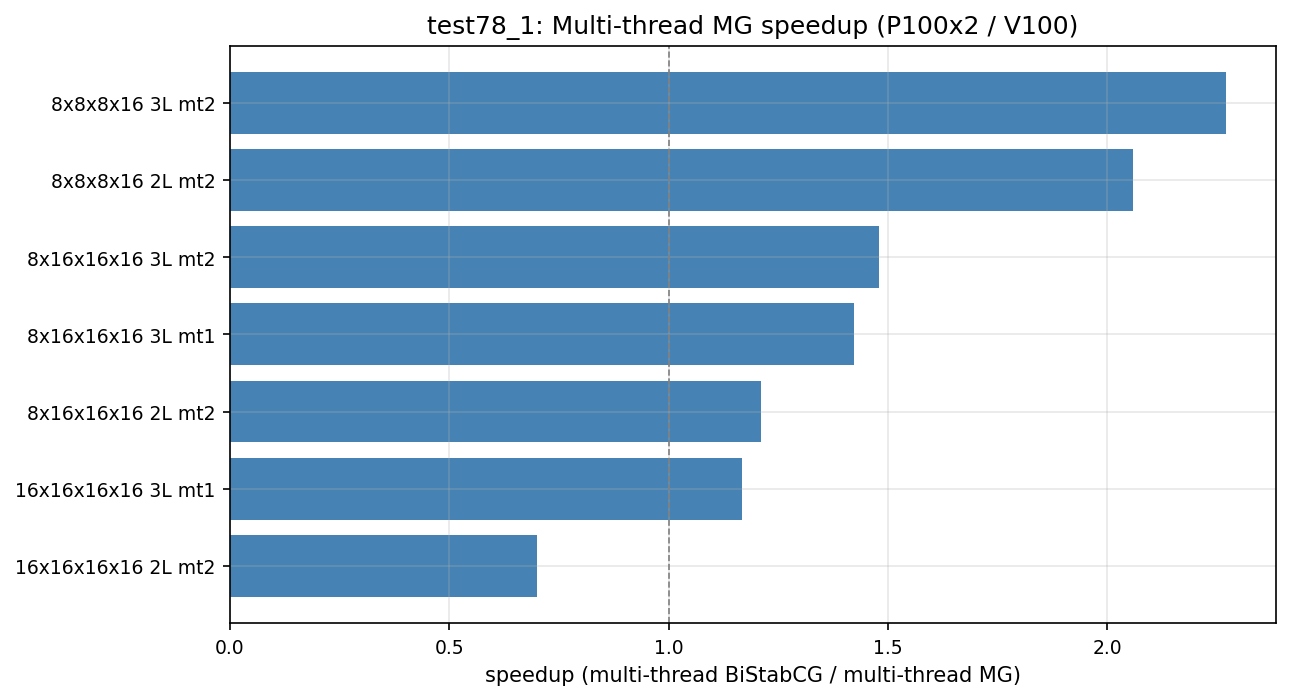
\includegraphics[width=0.9\textwidth]{../v202608160214/test78_1_speedup.png}
\caption{bench 加速比横条（test78\_1\_speedup.png）}
\end{figure}
\begin{figure}[htbp]\centering
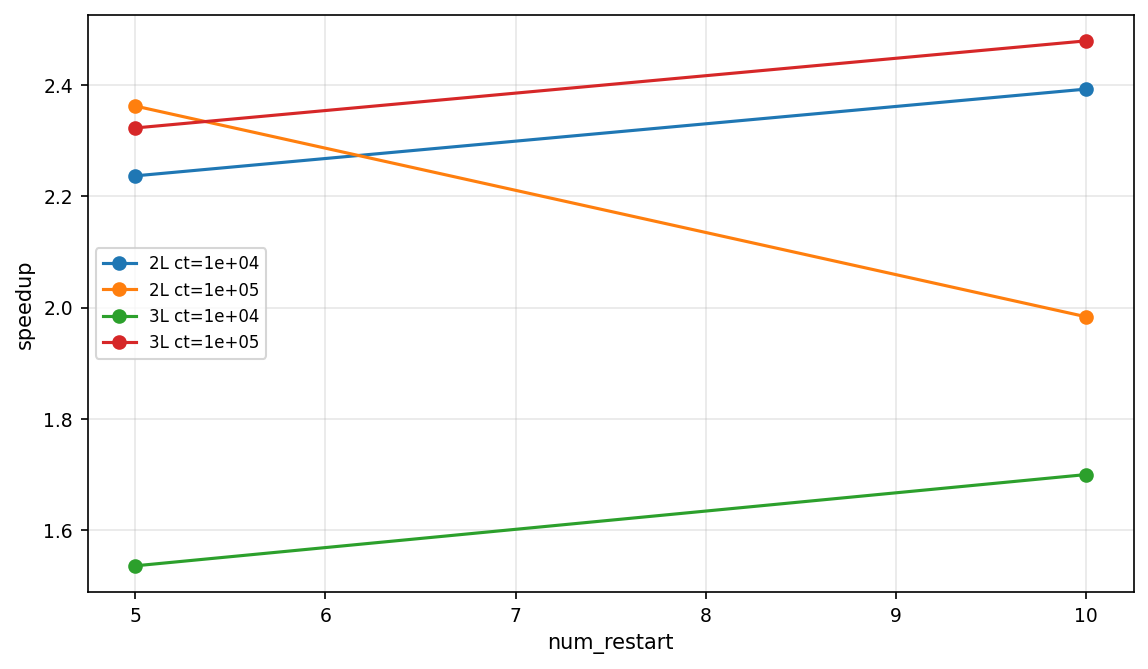
\includegraphics[width=0.9\textwidth]{../v202608160214/test78_1_sweep.png}
\caption{参数扫描 restart × speedup（test78\_1\_sweep.png）}
\end{figure}
\begin{figure}[htbp]\centering
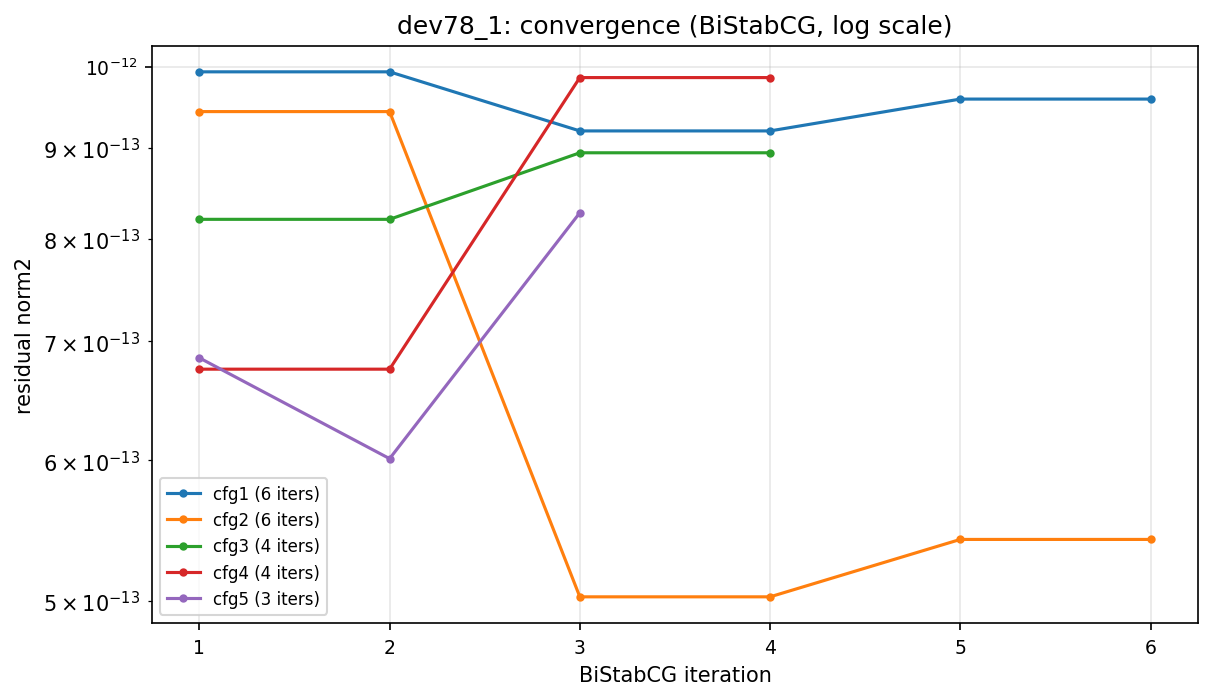
\includegraphics[width=0.9\textwidth]{../v202608160214/dev78_1_conv_bench.png}
\caption{BiStabCG 收敛曲线（dev78\_1\_conv\_bench.png，36 次求解）}
\end{figure}
\begin{figure}[htbp]\centering
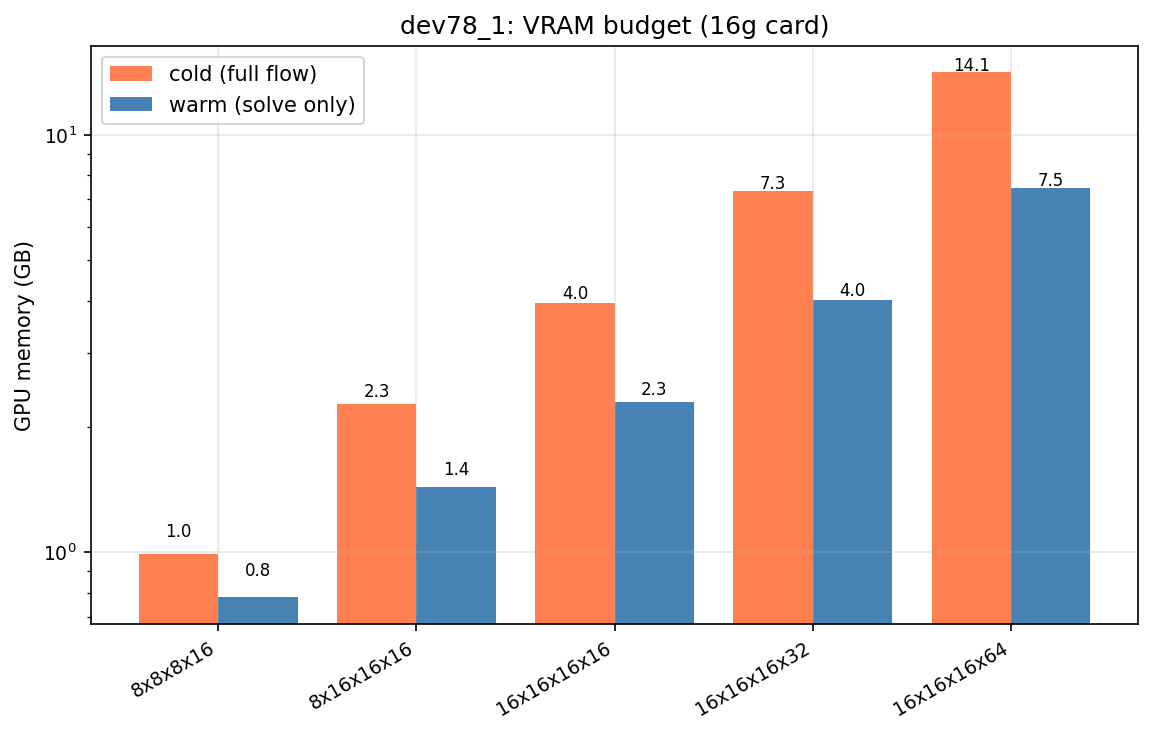
\includegraphics[width=0.9\textwidth]{../v202608160214/dev78_1_vram_16g.png}
\caption{显存预算（dev78\_1\_vram\_16g.png）}
\end{figure}
\begin{figure}[htbp]\centering
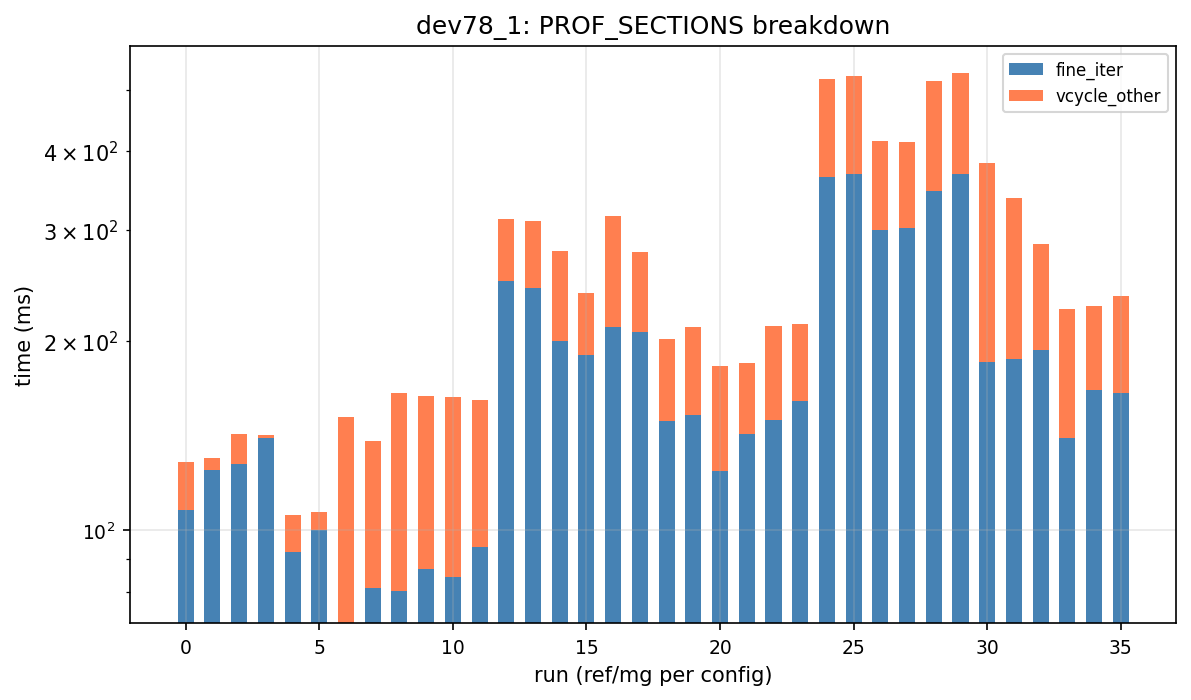
\includegraphics[width=0.9\textwidth]{../v202608160214/dev78_1_prof.png}
\caption{PROF\_SECTIONS 各段占比（dev78\_1\_prof.png）}
\end{figure}

% ================= 7 参考源清单 =================
\section{参考源清单}
\begin{xltabular}{\textwidth}{llX}
\toprule
\textcolor{evidence}{参考源} & 类型 & 内容/作用 \\
\midrule
\endhead
\texttt{\nolinkurl{logs/dev78_1/main.py:409-432}} & 仓库 & bench 配置（r10/r20） \\
\texttt{\nolinkurl{logs/dev78_1/v202608160214/test78_1_results.h5}} & 仓库 & 最终汇总数据 \\
\texttt{\nolinkurl{logs/dev78_1/v202608160214/bench.log}} & 仓库 & 收敛残差 + PROF \\
\texttt{\nolinkurl{logs/dev78_1/dev78_1_report.md}} & 仓库 & 详细报告 \\
\texttt{\nolinkurl{logs/dev78_1/AGENTS.md}} & 仓库 & 套件复现指南 \\
\texttt{\nolinkurl{logs/dev74/dev74.tex}} & 参考 & 输出形式参照 \\
\bottomrule
\end{xltabular}

% ================= 8 结论与局限 =================
\section{结论与局限}
\begin{conclbox}
三视角结论：\textcolor{struct}{结构}——套件 + 图表 + 日志三层完备；
\textcolor{relation}{关系}——num\_restart 控制粗层求解次数的性能主链；
\textcolor{idea}{思路}——实测闭环验证参数优化。
主题结论：dev78\_1 完整复测确认 r10/r20 优化——8x16x16x16 2L/3L 加速比
提升 2-3 倍并突破 1.0（1.41-1.48）；bench 中位 1.422 创里程碑新高；
verify 全 PASS、图表与日志全套归档。
\end{conclbox}
\begin{refbox}
dev74 的图表/日志/报告形式（收敛图、vram 图、budget 图、md+tex+pdf）
作为本套件输出规范；参数扫描（sweep）与资源预算（budget）为跨里程碑
可比性提供基础。
\end{refbox}
\begin{warnbox}
\textcolor{warn}{未验证}项：① 16x16x16x16 2L 仍 <1（0.74，层数固有）；
② 16x16x16x64 仅预算模型未实测（16G 上 88% 有风险）；③ 收敛图
（conv）基于 bench.log 的 LOOP 残差解析，多配置混合，单配置独立收敛
曲线未单独跑；④ r15 等中间值未扫（r10 与 r20 间最优未确认）。
\end{warnbox}

\end{document}
